\section{Methodology}
\label{sec:method}

\begin{figure*}[t]
    \centering
    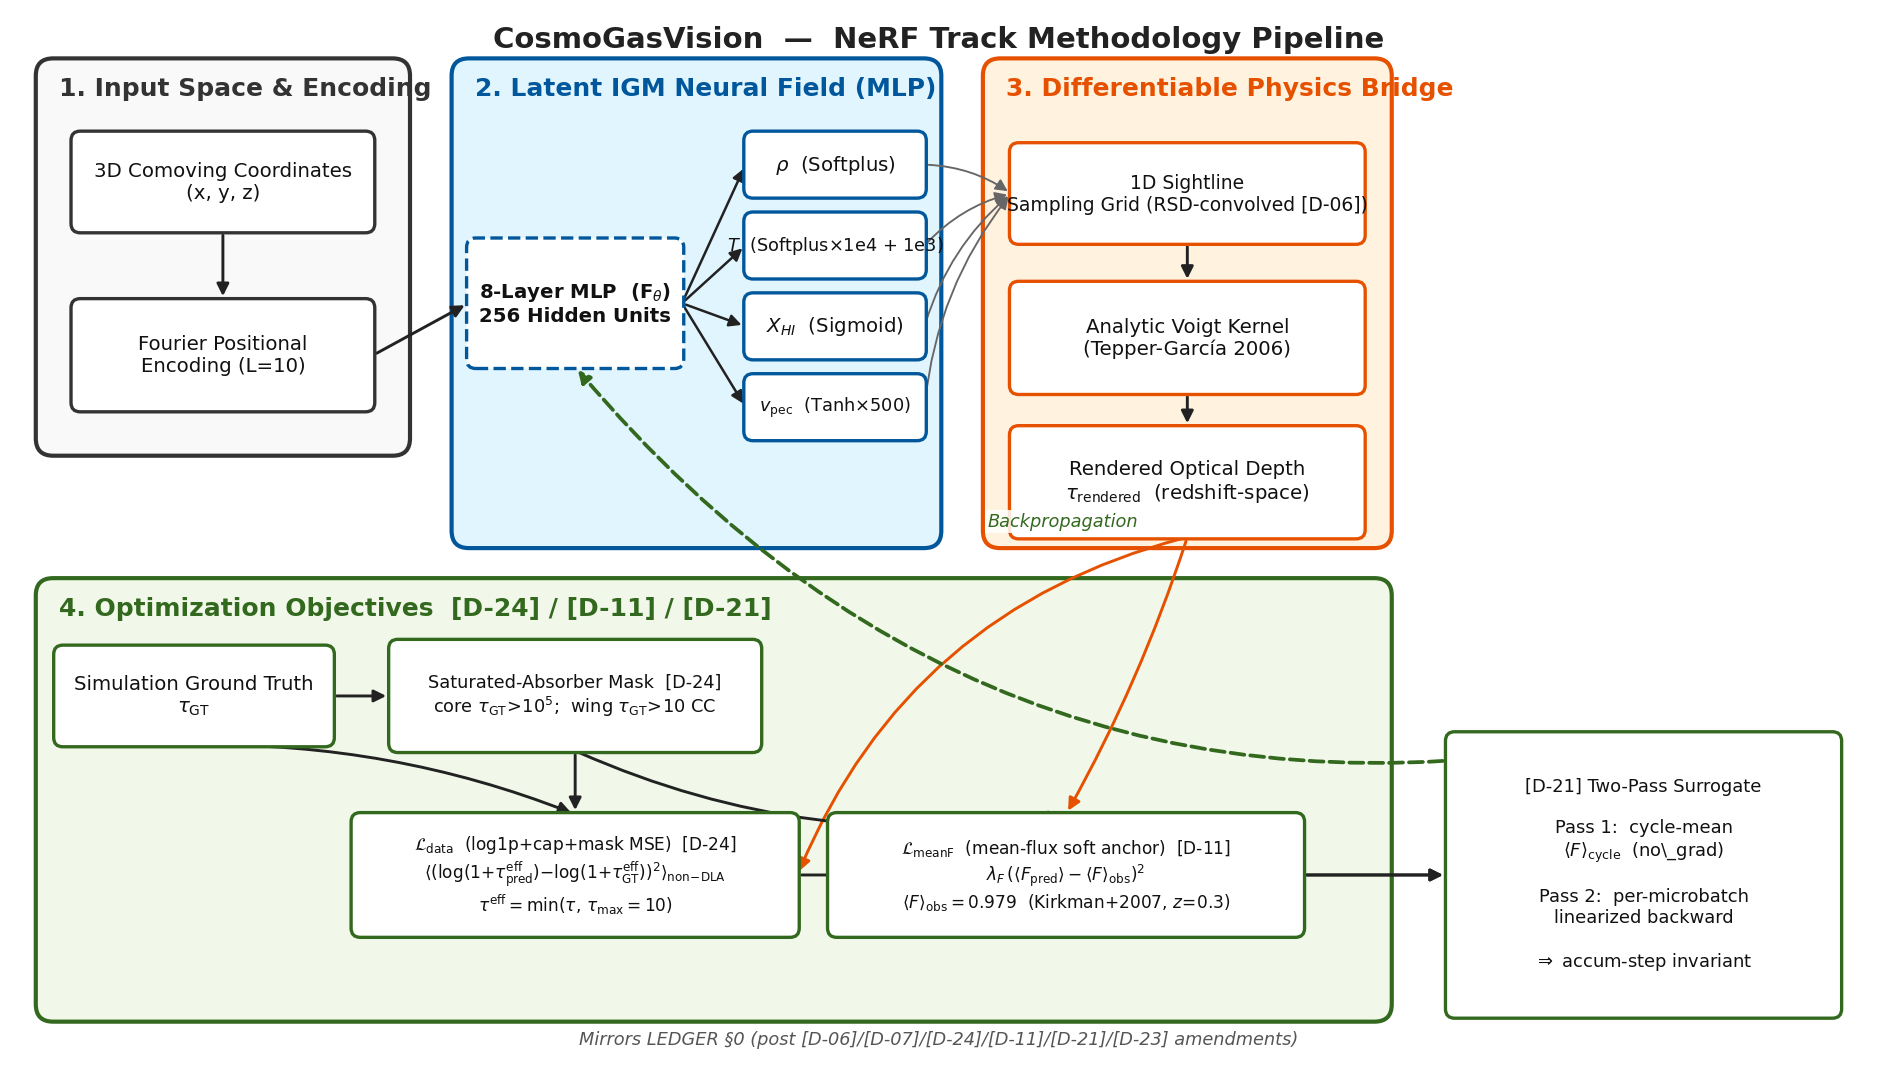
\includegraphics[width=0.80\textwidth]{figures/method_pipeline}
    \caption{The IGM-NeRF tomography pipeline. An 8-layer / 256-unit MLP (494{,}084 parameters) maps comoving 3D coordinates inside a 60 Mpc/h Sherwood box (normalized to $[0,1]^3$) through Fourier positional encoding ($L=10$) to four bounded astrophysical fields ($\rho/\bar\rho$, $T$, $X_{HI}$, $v_{\text{pec}}$). A differentiable RSD-convolved Voigt integrator with learnable amplitude $\mathcal{A}$ projects these fields to 1D optical depth $\tau(v)$, supervised against Sherwood ground truth under a log1p+cap+mask loss with the mean-flux anchor at $\langle F\rangle_{\text{obs}}(z=0.3) = \AnchorMeanF \pm \AnchorMeanFsigma$~\cite{kirkman2007}.}
    \label{fig:pipeline}
\end{figure*}

The core of \emph{CosmoGasVision} is an MLP $F_{\theta}: \mathbf{x} \to (\rho, T, X_{HI}, v_{\text{pec}})$, where $\mathbf{x} \in \mathbb{R}^3$ are comoving coordinates inside a 60 Mpc/h Sherwood box, normalized to $[0, 1]^3$. Fig.~\ref{fig:pipeline} shows the end-to-end pipeline: Fourier encoding, bounded-output MLP, RSD-convolved Voigt projection, and log1p+cap+mask supervision with the mean-flux anchor.

\subsection{Neural Field Architecture}
We adopt an 8-layer MLP with 256 hidden units per layer (494{,}084 parameters). To resolve the small-scale filamentary structures of the Cosmic Web, we use Fourier positional encoding~\cite{mildenhall2020nerf} $\gamma(\mathbf{x}) = (\sin(2^k\pi\mathbf{x}), \cos(2^k\pi\mathbf{x}))_{k=0}^{L-1}$ with $L=10$, sized to the $\sim\!100\times$ overdensity peaks of massive filaments.

\subsection{Bounded Physics Layer}
Final-layer activations enforce physical scales on each field: Softplus for $\rho/\bar\rho$ and $T$, Sigmoid for $X_{HI}\in[0,1]$, and scaled Tanh for $v_{\text{pec}}$ (exact scale constants in suppl.).

\subsection{Differentiable Physics Integrator}
The reconstruction is supervised by comparing rendered $\tau_{\text{rendered}}(v)$ against the simulation ground-truth $\tau_{GT}(v)$. The optical depth is an RSD convolution summing every source-bin's normalized line profile over every observed-velocity bin:
\begin{equation}
\tau(v_{\text{obs}}) = \mathcal{A} \sum_{\text{src}} n_{HI}^{\text{src}} \cdot \frac{H(a_{\text{src}}, x_{\text{src,obs}})}{b_{\text{src}}\sqrt{\pi}}
\end{equation}
where $x_{\text{src,obs}} = (v_{\text{obs}} - v_{\text{src}} - v_{\text{pec},\text{src}}) / b_{\text{src}}$, $b_{\text{src}}$ is the thermal Doppler parameter, and $\mathcal{A}$ is a learnable scalar absorbing $\sigma_0$, $ds$, and $\bar{n}_H$. The Voigt-Hjerting kernel uses the Tepper-Garc\'ia~\cite{tepper2006voigt} analytic approximation:
\begin{equation}
H(a, x) \approx e^{-x^2} - \frac{a}{\sqrt{\pi} x^2} \big[ e^{-2x^2} (4x^4 + 7x^2 + 4 + 1.5x^{-2}) - 1.5x^{-2} - 1 \big]
\end{equation}
allowing loss gradients to propagate back through the damping wings to the MLP parameters $\theta$. The integrator was audited end-to-end after a factor-12.9 damping-coefficient fix ([D-57]); the explicit-grid probe of \S\ref{sec:method:gridprobe} is supervised through the same forward model.

\subsection{Lyman-alpha Forest Loss: Saturated-Absorber Mask, Cap, and Log-Space Supervision}
\label{sec:method:loss}
A naive per-bin MSE on raw $\tau$ is dominated by rare saturated absorbers: damped Lyman-alpha systems (DLAs)~\cite{wolfe2005} and strong Lyman-limit systems~\cite{prochaska2010} produce $\tau_{\text{peak}} \sim 10^7$ in the Sherwood Physics-2/3/4 sightlines, four to five orders of magnitude above the diffuse forest. This saturation is forward-model-physical, not a label artifact, but carries no usable structure information for tomography because $F = e^{-\tau}$ is numerically zero in those bins. We therefore use \textbf{log-space supervision} (the methods contribution of this work) plus two \textbf{defense-in-depth} safeguards: a saturated-absorber detection mask (bins with $\tau_{GT}>10^5$ are flagged as saturated cores and expanded to the connected component of $\tau_{GT}>10$) and a forest cap ($\tau^{\text{eff}}=\min(\tau,\tau_{\max})$ with $\tau_{\max}=10$, calibrated against the Sec.~\ref{sec:experiments} gate and locked by a sensitivity sweep, see suppl.). The data loss on the surviving bins is
\begin{equation}
\mathcal{L}_{\text{data}} = \big\langle \big( \log(1 + \tau_{\text{pred}}^{\text{eff}}) - \log(1 + \tau_{GT}^{\text{eff}}) \big)^2 \big\rangle_{\text{non-saturated}}
\label{eq:data-loss}
\end{equation}
averaged over rays and unmasked velocity bins. The $\log(1+\tau)$ supervision space is physically motivated: Lyman-alpha-forest opacity is approximately log-normally distributed in $\tau$~\cite{bi_davidsen1997, hui_gnedin1997}, from FGPA $\tau \propto \rho^{1.6} T^{-0.7}$ on a near-log-normal density PDF. The mask and cap are defense-in-depth, not part of the novelty claim (see suppl.).

\subsection{Mean-Flux Anchor and Gradient Linearization}
The forward model is invariant under $\rho \to k\rho,\ \mathcal{A} \to \mathcal{A}/k$, so the data loss alone cannot fix the absolute overdensity amplitude. We break the degeneracy with the observational mean-flux constraint at $z = 0.3$:
\begin{equation}
\mathcal{L}_{\text{meanF}} = \lambda_F \big( \langle e^{-\tau_{\text{pred}}}\rangle - \langle F\rangle_{\text{obs}} \big)^2
\end{equation}
at $\langle F\rangle_{\text{obs}}(z=0.3) = \AnchorMeanF \pm \AnchorMeanFsigma$ from Kirkman et al.~\cite{kirkman2007}, with $\lambda_F = 1.0$. The Sec.~\ref{sec:experiments} cost-survey runs used an earlier broken anchor $0.877$; we retain them because the structure gates are anchor-invariant (calibration shifts only the absolute $\rho$ amplitude, not the structure-residual ratios). The constraint uses a two-pass surrogate to avoid \texttt{retain\_graph} in gradient accumulation; derivation in suppl.

\subsection{Training Configuration}
We optimize with AdamW under a tier-aware schedule (sightline count $n_{\text{rays}}$ rising T1 $64$ through T4 $16{,}384$, the highest tier deferred) with per-tier linear-warmup-then-cosine LR. Peak VRAM follows the validated linear model $\hat{V}_{\text{peak}}\approx\TonePeakVRAM\cdot\min(n_{\text{rays}},\mu\text{batch})/64$ GB (optimizer hyperparameters, per-tier step counts, and the VRAM table in suppl.).

\subsection{Explicit-Voxel-Grid Probe}
\label{sec:method:gridprobe}
The MLP couples its four fields through a shared body, so a failure to recover structure could be a capacity limit of the implicit representation rather than a property of the inverse problem. We separate the two with an explicit-voxel-grid probe: we replace $F_\theta$ with four independent free-per-voxel grids at resolution $\GridG^3$ (one grid per field, no shared body, no encoding bandwidth limit) and train them under the same forward model and the same flux supervision as the MLP. This is the maximal-capacity parameterization within this study --- the most degrees of freedom and the least regularization we give the problem; the single lever is the per-voxel field values, so the optimizer can place any value at any voxel. Hash-grid or multiresolution conditioning is a separate, untested axis. The probe asks one question: given a representation with enough capacity to fit any field, does the flux supervision identify the true 3D field?
